%!TEX root = ../main.tex
\chapter{Introduzione}\label{chp:introduction}

Ad oggi l'avanzamento della genomica — branca della biologia molecolare che si occupa di studiare il genoma degli esseri viventi — si è rivelato notevolmente significativo al fine di approfondire e comprendere malattie legate alle mutazioni del genoma degli individui. Si stima che solamente una percentuale tra l'1\% e il 2\% del DNA contiene i \textsl{geni}, ovvero particolari regioni che contengono tutte le informazioni necessarie per la sintesi degli aminoacidi che poi comporranno le proteine\,\cite{sahu2011identification, pollard2022cell}. Ciò nonostante, la quasi totalità dei disturbi genomici è dovuta alle mutazioni nelle regioni non codificanti\,\cite{zhang2015non} — dette \textsl{varianti non codificianti}. Le mutazioni in queste zone del genoma, che apparentemente svolgono funzioni marginali, sono responsabili dello sviluppo di disturbi importanti, come le \textsl{malattie mendeliane}\footnote{Le malattie mendeliane, causate dalla mutazione di un singolo gene, includono la fibrosi cistica e il morbo di Huntington.}\,\cite{french2020role, chial2008mendelian}, l'epilessia\,\cite{pagni2022non}, malattie cardiovascolari\,\cite{kapoor2014enhancer, zhang2015non} e soprattuto tumori — tra cui il cancro del colon-retto e tumore al seno\,\cite{khurana2016role, tian2019systematic, bojesen2013multiple, michailidou2017association}.

Risulta quindi vitale continuare a studiare gli effetti che le varianti non codificanti in sequenze genomiche hanno sugli individui. Proprio a questo proposito, con l'avvento dell'intelligenza artificiale, in particolare del \textsl{deep learning}, si continuano a trovare e perfezionare soluzioni che permettano di delineare sempre con più precisione il ruolo che hanno le mutazioni nelle regioni non codificanti del DNA.\@ Grazie a queste nuove tecnologie, la \textsl{genomica funzionale} — area della genomica che si interessa a descrivere le relazioni che ci sono tra i componenti di un sistema biologico, come geni e proteine\,\cite{caudai2021ai} — ha avuto un forte impulso nell'approfondire le varianti non codificanti ma rimangono ancora significative lacune nella comprensione riguardante la relazione tra mutazioni genetiche ed espressione genica. L'utilizzo di tecniche di deep learning quindi cruciale per continuare la ricerca; a questo proposito, nel presente elaborato accademico verranno descritti e paragonati tre \textsl{tool} che utilizzano le \textsl{reti neurali convoluzionali} per predire l'effetto delle varianti non codificanti su sequenze genomiche: DeepSEA\,\cite{zhou2015predicting}, Basset\,\cite{kelley2016basset} e DeepSATA\,\cite{ma2023deepsata}.



\section{Background}

La cellula è l'unità fondamentale della vita. La cellula è una piccola miscela acquosa con componenti chimici, racchiusi in una mambrana, e possiede l'eccezionale capacità di replicarsi. Il primo elemento che permette di distinguere le cellule è la presenza di un nucleo. Vengono definite \textsl{procarioti} le cellule senza nucleo — che sono le più diffuse e compongono organismi unicellulari come i batteri e gli archei — mentre sono chiamate \textsl{eucarioti} le cellule che contengono un nucleo — le quali sono in genere più grandi e più complesse e costituiscono forme di vita multicellulari come animali piante e funghi\,\cite{alberts2015essential}.

All'interno della cellula eucariote (illustrazione\,\ref{fig:cell}), immersi nel \textsl{citoplasma}, sono presenti diversi \textsl{organuli}, i quali svolgono una particolare funzione ciascuno. I \textsl{mitocondri} sono gli organuli più diffusi all'interno del \textsl{citoplasma}. Il loro compito è quello di generare energia chimica per la cellula: attraverso il processo di ossidazione di zuccheri e grassi, viene creata una sostanza che viene utilizzata nella maggior parte delle attività cellulari\footnote{Questa sostanza è detta \textsl{adenosintrifosfato} o ATP ed ha una struttora simile ad un nucleotide: è infatti composta dall'Adenina, da uno zucchero e da tre gruppi fosfati.}; questo processo è anche chiamato \textsl{respirazione cellulare} perchè consumando l'ossigeno viene rilasciata anidride carbonica\,\cite{alberts2015essential, chinnery2003mitochondria}. Oltre ad essere la fonte energetica primaria della cellula, i mitocondri hanno anche importanti ruoli nella regolazione del metabolismo, del ciclo cellulare, delle risposte antivirali e anche della morte della cellula\,\cite{mcbride2006mitochondria}.

\begin{figure}[b!]
    \centering
    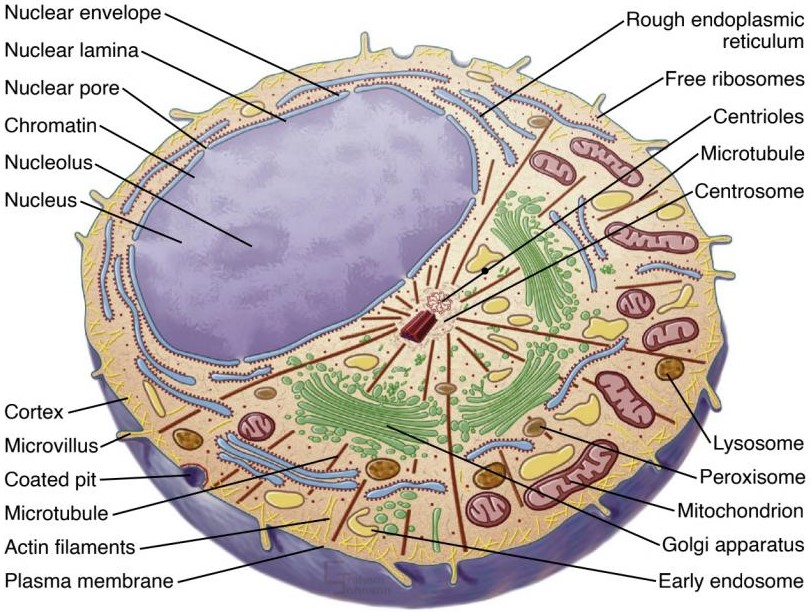
\includegraphics[width=.65\textwidth]{assets/cell.jpg}
    \caption[Rappresentazione schematica della cellula eucariote.]{Rappresentazione schematica della cellula eucariote; si possono notare i principali organuli tra cui i mitocondri, lisosomi e perossiomi, il reticolo endoplasmatico, e il nucleo\,\cite{pollard2022cell}.}\label{fig:cell}
\end{figure}

Il \textsl{reticolo endoplasmatico} è invece un organulo molto esteso e svolge molteplici funzioni. Tra queste compiti rientrano quelli di traslocazione di proteine e il ripiegamento delle proteine (\textsl{protein folding})\,\cite{alberts2015essential, voeltz2002structural}. I \textsl{lisosomi} si occupano di degradare e riciclare gli scarti cellulari e giocano un ruolo fondamentale per l'omeostasi della cellula\footnote{Con omeostasi cellulare si intende l'insieme di meccanismi necessari per mantenere ad un livello ottimale le funzioni della cellula.}, il suo sviluppo e il suo invecchiamento\,\cite{ballabio2016awesome, yang2021lysosome, dell2000lysosome}. Infine, i \textsl{perossiomi} sono delle piccole vescicole che forniscono un ambiente protetto per gestire molecole tossiche come gli acidi grassi i quali sono smaltiti tramite la $\beta$-ossidazione\,\cite{alberts2015essential, islinger2012peroxisome, islinger2018peroxisome}.

L'organulo più importante della cellula rimane il \textsl{nucleo}. Racchiuso nell'\textsl{involucro nucleare}, all'interno di questo organulo sono presenti tutte le informazioni genetiche, racchiuse in una lunga molecola di acido desossiribonucleico (comunemente noto come DNA), che, una volta impacchettato forma il \textsl{cromosoma}\,\cite{pollard2022cell, alberts2015essential}. La molecola di DNA è una struttura a doppia elica formata da \textsl{nucleotidi}. Osservando l'illustrazione\,\ref{fig:dna}, i nucleotidi sono composti a loro volta da tre elementi fondamentali: una \textsl{base azotata}, uno \textsl{zucchero} e un \textsl{gruppo fosfato}\footnote{I gruppi fosfati hanno una carica negativa e forniscono alla molecola le proprietà di un acido.}. Le basi azotate sono quattro — Adenina (A), Citosina (C), Guanina (G) e Timina (T) — e si uniscono tra loro mediante dei legami ad idrogeno e secondo un preciso criterio: l'Adenina si lega solamente con la Timina (formando il legame \textit{AT}) mentre la Citosina si unisce solo con la Guanina (creando la coppia \textit{CG})\,\cite{fonseca2000hydrogen, sahu2011identification}. Si osserva infine che il nucleotide di una coppia e quello successivo si legano mediante zucchero e gruppo fosfato sempre allo stesso modo: il gruppo fosfato di un nucleotide si lega sempre allo zucchero dell'altro. Di conseguenza, preso un filamento della doppia elica, le due estremità non sono uguali in quanto una termina con un gruppo fosfato (terminazione $5^\prime$) e l'altra con uno zucchero (terminazione $3^\prime$).

\begin{figure}[b!]
    \centering
    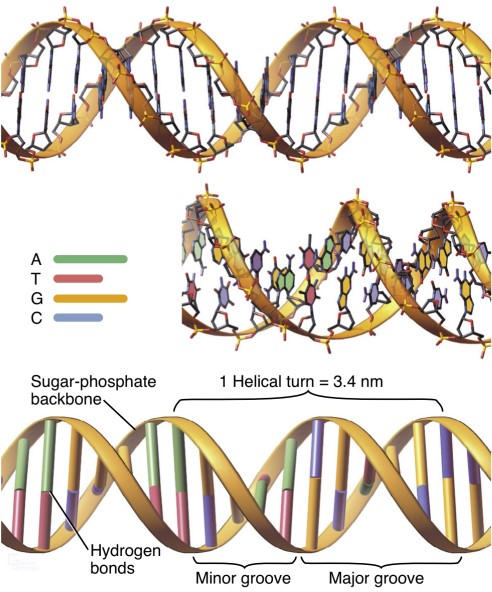
\includegraphics[width=.5\textwidth]{assets/dna.jpg}
    \caption[Rappresentazione schematica del DNA.]{Rappresentazione schematica del DNA;\@ si possono osservare le coppie di basi azotate, legate tra loro attraverso gli zuccheri e i gruppi fosfati\,\cite{pollard2022cell}.}\label{fig:dna}
\end{figure}

Attraverso una serie di ripiegamenti, una molecola di DNA lunga circa due metri riesce a raggomitolarsi in un cromosoma di grandezza inferiore a 2 micron (figura\,\ref{fig:dna-packaging}). Il processo di \textit{DNA-packaging} inizia avvolgendo la doppia elica di DNA attorno a delle proteine dette \textsl{istoni} e formado dei \textsl{nucleosomi}. In secondo luogo i nucleosomi si ammassano vicini tra loro formando una fibra, chiamata \textsl{cromatina} che, a sua volta si impacchetta su se stessa creando il cromosoma\,\cite{jansen2011nucleosome, zheng2010packaging}.

\begin{figure}[b!]
    \centering
    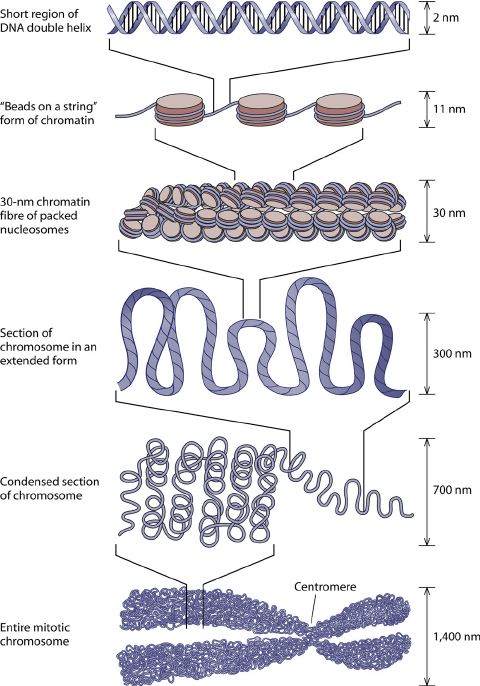
\includegraphics[width=0.6\textwidth]{assets/dna-packaging.png}
    \caption[Il processo di impacchettamento del DNA.]{Il processo di impacchettamento del DNA\,\cite{jansen2011nucleosome}.}\label{fig:dna-packaging}
\end{figure}

La rilevanza del DNA è data delle informazioni essenziali che questa molecola contiene. Tali informazioni risiedono nei geni, che sono delle sequenze genomiche che codificano uno o più prodotti biologici operativi\,\cite{gerstein2007gene}. L'\textsl{espressione genica} è il processo che permette di utilizzare i dati contenuti nel gene per la creazione di macromolecole, come le proteine. Per esempio, le cellule della pelle a contatto con luce solare intensa possono esprimere geni che regolano la pigmentazione della pelle\,\cite{white2009gene}. L'espressione genica è divisa in due fasi principali: la \textsl{trascrizione} — che si occupa di produrre delle molecole di RNA che rispecchino il gene da esprimere — e la \textsl{traduzione} — la quale traduce le informazioni dell'RNA sintetizzando la proteina.

Nella prima fase dell'espressione genica, è necessario trascrivere il DNA in una molecola molto simile ovvero l'RNA — chiamato anche acido ribonucleico. Questa molecola differisce dall'acido desossiribonucleico per una base azotata — anzichè la Timina è presente l'Uracile (U) — e per lo zucchero — da desossiribosio a ribosio\,\cite{alberts2002dna}. La trascrizione del DNA in RNA inizia quando delle proteine, chiamate \textsl{fattori di trascrizione}, riconoscono la regione che delimita l'inizione della molecola del gene da esprimere, detta \textsl{zona promotrice}. Dopo aver riconosciuto l'inizio della sequenza, queste proteine permettono ad un enzima chiamata \textsl{RNA polimerasi} di attaccarsi ed aprire la doppia elica del DNA\,\cite{cramer2019organization}. Una volta aperta la doppia elica, inizia la vera e propria trascrizione in RNA:\@ il filamento del DNA viene preso come modello per la creazione dell'RNA;\@ in particolare il nucleotide dell'RNA sarà il complementare rispetto a quello del DNA (di conseguenza $A\to U$, $C\to G$, $G\to C$ e $T\to A$). Così facendo l'acido ribonucleico viene creato un nucleotide alla volta, analizzando quello del DNA\,\cite{alberts2002dna}. La trascrizione termina nel momento in cui gli enzimi e le proteine incontrano la regione terminatrice del gene che determina la separazione dal filamento e la terminazione dell'RNA \textsl{messaggero} (\textsl{mRNA}) che contiene le informazioni presenti nel gene da esprimere. L'intero processo di trascrizione è illustrato nella figura\,\ref{fig:gene-transription}.

\begin{figure}[b!]
    \centering
    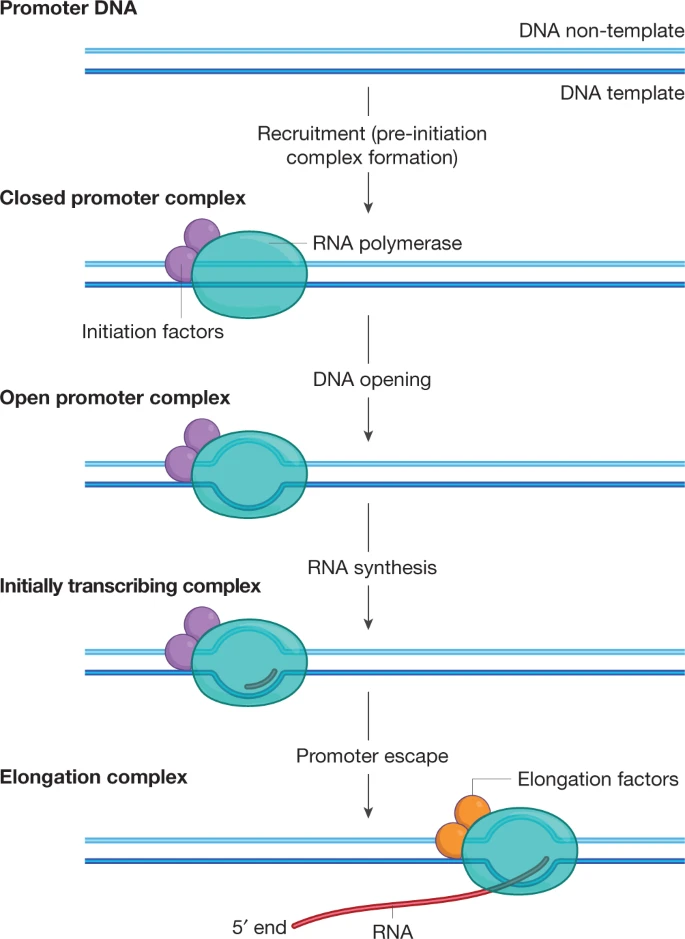
\includegraphics[width=0.6\textwidth]{assets/gene-transcription.png}
    \caption[Il processo di trascrizione del DNA del gene in RNA.]{Il processo di trascrizione del DNA del gene in RNA\,\cite{cramer2019organization}.}\label{fig:gene-transription}
\end{figure}

Prima di uscire dal nucleo l'RNA messaggero subisce una serie di elaborazioni necessarie per rendere le informazioni immagazzinae sicure: diverse sono le malattie che emergono per mutazioni presenti nell'mRNA tra cui la distrofia miotonica\footnote{Le distrofie miotoniche sono patologie che colpiscono principalmente l'apparato muscolo-scheletrico.}\,\cite{philips2000rna}. La prima eleborazione viene chiamata $5^\prime$-\textit{end capping} e si occupa di aggiungere alla terminazione $5^\prime$ dell'mRNA una Guanina attraverso un collegamento inusuale che garantisce maggiore stabilità alla molecola. In secondo luogo avviene lo \textit{splicing} che si occupa di rimuovere le zone non-codificanti — dette \textsl{introni}— dal gene trascritto mantenendo solo quelle che verranno utilizzate per essere sintetizzate in proteine — gli \textsl{esoni} — e quindi facilitando il processo di traduzione. Infine con il $3^\prime$-\textit{end processing} viene aggiunta alla terminazione $3^\prime$ dell'mRNA una coda di Adenine — datta anche \textit{poly}A \textit{tail} — che, in maniera molto simile al $5^\prime$-\textit{end capping} garantisce una stabilità del filamento di acido ribonucleico\,\cite{hocine2010rna}.

Dopo essere uscito dal nucleo, l'mRNA è pronto per essere tradotto in proteina.

\todo{Informazioni contenute nel DNA, funzione del dna del creare proteine. I \textsl{ribosomi} si occupano di accelerare la sintesi delle proteine usando le sequenze di nucleotidi del \textsl{RNA messaggero} (mRNA) per specificare la sequenza di aminoacidi\,\cite{fortin2015trx, stormo1998specificity, travers2015dna}}
\todo{geni, parti del gene in modo da spiegare bene le varianti non codificanti}

\todo{Parla dei nucleoli\,\cite{pederson1998plurifunctional}}

\todo{Come accennato all'inizio del capitolo, la cellula possiede la notevole capacità di replicarsi; il processo replicazione cellulare è detto \textsl{mitosi}.}
\todo{DNA replication\,\cite{bell2002dna} durante il ciclo della mitosi (non descriverla tutta) \,\cite{mcintosh2012biophysics}}

\section{Cenni storici}
\todo{
    C'è sto bell'articolo che racconta per bene la situa\cite{crick1954complementary, watson1953molecular, li2021cell}. Qua ci puoi buttare dentro anche la questione meme del junk DNA così pushi per bene le citazioni goliardiche. Cita il libro\,\cite{pollard2022cell} che descivre a cosa serve il dna (pagina 10)
}
\todo{ Sto libro parla anche della scopetrta delle cellule\cite{alberts2015essential}}


\section{Stato dell'arte}

\todo{parla dei tool e quanti ne sono uscit per letsgoscare le cose. Parla delle diversi vantaggi che AI ha portato nel letsgosky. Butta dentro deepvirfinder a anche alphafold perche fa figo\cite{ren2020identifying}}
\todo{anche esmpi di DNA folding}


% https://books.google.it/books?hl=it&lr=&id=Cg4WAgAAQBAJ&oi=fnd&pg=PP1&dq=Introduction+to+cell+biology&ots=yg4LdM46O3&sig=FkW8Ei_rOFccb96Sw3A28QsHuFo&redir_esc=y#v=onepage&q=Introduction%20to%20cell%20biology&f=false

% https://books.google.it/books?hl=it&lr=&id=mXiiEAAAQBAJ&oi=fnd&pg=PP1&dq=cellular+biology&ots=8O1TrOZBXp&sig=fqZhVnT0H-I3qEu1iPk4v2nvZi8&redir_esc=y#v=onepage&q=cellular%20biology&f=false

% https://books.google.it/books?hl=it&lr=&id=z4BDRcLrekMC&oi=fnd&pg=PR19&dq=cell+nucleus+organization&ots=wiXN8JbVpC&sig=oviVqMKJqsvcYwe4X37tQM28P3Y&redir_esc=y#v=onepage&q=cell%20nucleus%20organization&f=false
